\documentclass[sensors,article,submit,moreauthors,pdftex]{Definitions/mdpi}

\firstpage{1}
\makeatletter
\setcounter{page}{\@firstpage}
\makeatother
\pubvolume{xx}
\issuenum{1}
\articlenumber{5}
\pubyear{2026}
\copyrightyear{2026}
\history{Received: date; Accepted: date; Published: date}

\graphicspath{{figures/}}
\DeclareGraphicsExtensions{.pdf,.png,.eps}

\usepackage{amsmath}
\usepackage{booktabs}
\usepackage{subcaption}
\usepackage{multirow}
\usepackage{siunitx}
\setlength{\emergencystretch}{2em}

\Title{AERIS: Environment-Aware Hierarchical Routing for Reliable Wireless Sensor Networks under Realistic Channel Conditions}

\Author{Kangrui Li $^{1,}$*, Xiaobo Zhang $^{1}$ and Junyi Lin $^{1}$}
\AuthorNames{Kangrui Li, Xiaobo Zhang and Junyi Lin}
\address{$^{1}$ \quad Faculty of Automation, Guangdong University of Technology, Guangzhou 510006, China}
\corres{Correspondence: 1403073295@mails.gdut.edu.cn}

\abstract{This paper presents AERIS, an environment-aware hierarchical routing protocol for wireless sensor networks, and evaluates it with \texttt{pdr\_expected} as the primary metric. In the publication-tier 100-node matrix (four environments, 30 seeds per environment), AERIS attains the highest mean PDR within the tested baseline set (LEACH, PEGASIS, HEED, TEEN). In the balanced S8 scalability matrix (100--1000 nodes, four environments, 1000 replicates per environment-node-protocol cell), AERIS remains first by mean PDR in all 24 environment-scale cells; however, this matrix is treated as baseline evidence because the original path omits explicit MAC-collision penalties and shows non-physical upward trends in three environments. We therefore use S9/S10/S11 as rigor-calibration blocks under stricter assumptions. S10 (tx-power 5 vs 15 dBm, n=600 per cell) yields significant differences in 59/60 cells after Holm correction. In the matched S11 matrix (patch n=1000, control n=1000), AERIS patch-control deltas are negative and significant in all 24 environment-scale cells, indicating reliability degradation under the current collision/relay patch configuration. NS-3 is used for cross-platform trend validation (AERIS vs LEACH) and is explicitly reported as trend-level evidence rather than numerical-equivalence proof.}

\keyword{wireless sensor networks; reliable routing; hierarchical protocol; packet delivery ratio; scalability; reproducible evaluation}

\begin{document}

\section{Introduction}
Wireless sensor network (WSN) routing is classically optimized for energy reduction, but practical deployments also require stable delivery under heterogeneous channels \cite{Akyildiz2002Survey,Rault2016Energy,Kandris2020}. This creates a multi-objective tension among reliability, hop-based latency, and energy use. Existing protocols represent distinct operating points: LEACH emphasizes clustered forwarding \cite{Heinzelman2000LEACH}, PEGASIS emphasizes chain-based aggregation \cite{Lindsey2002PEGASIS}, HEED emphasizes residual-energy-aware head selection \cite{Younis2004HEED}, and TEEN emphasizes event-triggered reporting \cite{Manjeshwar2001TEEN}. Prior channel studies also show that low-power links can be asymmetric and environment-sensitive under realistic propagation conditions \cite{Zuniga2004,Zuniga2007Asymmetry,Baccour2012RLQE}.

AERIS is designed as a lightweight hierarchical protocol that prioritizes reliability under realistic channel variability. The design objective is not universal dominance; rather, it is robust performance across multiple channel environments while preserving deployability on resource-constrained nodes.

\subsection*{Contributions and Scope Boundaries}
This manuscript makes three scoped contributions:
\begin{itemize}
\item a modular routing design (CAS switching, Skeleton backbone, Gateway reinforcement) with explicit environment-scoped operation boundaries and auditable control variables;
\item publication-tier evidence matrices that separate core reliability reporting (100-node + frozen S8 matrix) from physics-calibration blocks (S9/S10/S11), avoiding cross-regime over-aggregation;
\item cross-platform NS-3 trend validation for AERIS versus LEACH under aligned environment taxonomy, with strict trend-level reporting boundaries.
\end{itemize}
The manuscript focuses on reproducible conclusions under explicit settings (metric, environment taxonomy, baseline set, and sample-size design) and does not claim cross-platform numerical equivalence.

\section{Related Work}
Classical WSN protocols (LEACH, PEGASIS, HEED, TEEN) provide foundational routing mechanisms but show different failure modes under harsh channels and larger scales \cite{Heinzelman2002LEACH,Lindsey2002PEGASIS,Younis2004HEED,Kandris2020}. Chain-based aggregation can reduce per-hop transmission effort but increases end-to-end hop count. Cluster-based approaches can reduce hop count but may become sensitive to uplink quality and head placement.

Recent adaptive or learning-based methods improve specific settings but often require heavier runtime or training overhead \cite{Ren2024,Okine2024,Chen2019Survey}. Recent Sensors/IoT studies also report robust gains from context-aware or hybrid routing under constrained networks \cite{ElFouly2023ILP,Dan2024EMRAR,Bhukya2025Hybrid}. These results motivate explicit environmental adaptation in protocol design while keeping inference and control logic lightweight. In this manuscript, the focus is a rule-based protocol with explicit reproducibility constraints and auditable experiment metadata.

\section{System Model and Protocol}
\subsection{Metric Definition}
The primary metric is
\begin{equation}
\mathrm{PDR}_{\mathrm{expected}} = \frac{\mathrm{bs\_delivered}}{\mathrm{source\_packets\_expected}}.
\end{equation}
All publication conclusions in this draft are based on this metric.

\subsection{AERIS Architecture}
AERIS combines three components:
\begin{enumerate}
\item Context-Adaptive Switching (CAS) for mode control,
\item Skeleton backbone for hierarchical forwarding,
\item Gateway coordination for CH-to-BS reinforcement.
\end{enumerate}
Gateway candidate scoring follows a weighted rule
\begin{equation}
\mathrm{Score}_i = \alpha E_i + \beta C_i + \gamma L_i
\end{equation}
where $E_i$ is residual energy, $C_i$ is centrality, and $L_i$ is link quality.
CAS mode selection is modeled as
\begin{equation}
m^{*}=\arg\max_{m\in\{\mathrm{direct},\mathrm{chain},\mathrm{twohop}\}}
\left(w_{1,m}\hat{q}_{m}+w_{2,m}\hat{e}_{m}+w_{3,m}\hat{u}_{m}+b_m\right),
\end{equation}
where $\hat{q}_{m}$, $\hat{e}_{m}$, and $\hat{u}_{m}$ are normalized link-quality, energy, and uncertainty features for mode $m$.

\subsection{Round-Level Operation}
Each simulation round follows a fixed sequence: (i) cluster-head election and clustering, (ii) intra-cluster delivery with CAS mode selection, (iii) CH-to-BS forwarding with optional Gateway/Skeleton support, and (iv) metric logging. This ordering is held constant across protocols to preserve comparability in the reported matrices.

\section{Experimental Setup}
\subsection{Publication-Tier Settings}
\begin{itemize}
\item Simulator: Python implementation with logged provenance.
\item Channel environments: indoor\_office, indoor\_factory, outdoor\_urban, outdoor\_suburban.
\item Default node count: 100.
\item Seeds for multi-environment and ablation: 30 independent seeds.
\item Seeds for scalability: balanced frozen regime with n=1000 per environment-node-protocol cell (100--1000 nodes, 4 environments).
\item Baselines: LEACH, PEGASIS, HEED, TEEN.
\end{itemize}

\subsection{Evidence Scope}
The analysis is grounded in publication-tier multi-environment comparison, ablation, scalability, hop-based latency, energy-lifetime statistics, and NS-3 trend validation. Cross-regime numerical pooling is avoided.

\subsection{Simulator Regimes and Physics Assumptions}
This study reports two simulation regimes for scalability interpretation. The frozen S8 regime is the original simulator path used for the balanced 100--1000 node matrix. The S9/S10/S11 regime introduces stricter-physics controls (collision/relay stress, matched patch-control checks, and tx-power sensitivity) and is used for calibration and boundary checks. We therefore do not pool S8 and S9/S10/S11 values into a single headline estimate. Instead, S8 is treated as the baseline reporting matrix, while S9/S10/S11 are treated as rigor-calibration blocks that quantify how conclusions shift under stricter assumptions.

\begin{table}[H]
\caption{Evidence-regime map used in this manuscript.}
\label{tab:regime_map}
\centering
\resizebox{\linewidth}{!}{
\begin{tabular}{llll}
\toprule
Block & Scope & Typical sample size & Role in claims \\
\midrule
100-node matrix & 4 env $\times$ 5 protocols & n=30 per env-protocol cell & Core reliability comparison \\
S8 scalability & 4 env $\times$ 6 node counts $\times$ 5 protocols & n=1000 per env-node-protocol cell & Baseline large-scale matrix \\
S9 patch-control & 4 env $\times$ 6 node counts $\times$ 5 protocols & patch n=1000, control n=600 & Physics-stress calibration \\
S10 power sensitivity & 4 env $\times$ 3 node counts $\times$ 5 protocols & n=600 per env-node-protocol cell & Tx-power boundary analysis \\
S11 matched patch-control & 4 env $\times$ 6 node counts $\times$ 5 protocols & patch n=1000, control n=1000 & Matched strict-physics confirmation \\
NS-3 alignment & 4 env $\times$ 7 node counts, AERIS vs LEACH & n=30 per env-node-protocol cell & Trend-level cross-platform check \\
\bottomrule
\end{tabular}
}
\end{table}

\subsection{Statistical Methods}
For pairwise protocol comparisons, we use Welch's two-sample $t$-test:
\begin{equation}
t=\frac{\bar{x}_1-\bar{x}_2}{\sqrt{\frac{s_1^2}{n_1}+\frac{s_2^2}{n_2}}},
\end{equation}
because variance equality is not assumed across protocols and environments. Family-wise error control is handled by Holm correction within each reported comparison family. Effect size is reported with Hedges' $g$:
\begin{equation}
g = J\cdot\frac{\bar{x}_1-\bar{x}_2}{s_p},\quad
J=1-\frac{3}{4(n_1+n_2)-9},
\end{equation}
and interpreted as small (0.2), medium (0.5), and large (0.8) in absolute value. Confidence intervals are reported as two-sided 95\% intervals. All significance statements in this manuscript are based on Holm-corrected $p$ values. For large-$n$ cells, interpretation is based jointly on corrected $p$ values, effect size, and absolute PDR delta. Reported table-wise standard deviations are treated as descriptive values from the corresponding result files; inferential conclusions are computed from raw replicate-level records.

\subsection{Reproducibility Controls}
All publication-tier scripts in this study use deterministic seed lists. They also enforce \texttt{force\_ctp\_reliable=False}. This guarantees that PDR reflects simulated delivery behavior rather than any reliability override. We report \texttt{pdr\_expected} as the primary metric and treat hop count as a latency proxy, not a wall-clock latency measurement. Significance statements are accepted only when consistent with the declared regime-specific sample size.

\subsection{Auditability Constraints}
To keep claims machine-checkable, each publication-tier output includes run-tier tags, metric tags, and script/hash sidecar metadata. Claims in the main text are restricted to matrices that satisfy declared sample-size and metric constraints. This prevents mixing exploratory diagnostics with publication-tier statements.

\section{Results}
\subsection{Multi-Environment Comparison at 100 Nodes (n=30)}
\begin{table}[H]
\caption{PDR by environment at 100 nodes (mean $\pm$ std; standard deviations are reported as stored in the source result file).}
\label{tab:pdr100}
\centering
\resizebox{\linewidth}{!}{
\begin{tabular}{lccccc}
\toprule
Environment & AERIS & LEACH & PEGASIS & HEED & TEEN \\
\midrule
indoor\_office   & 0.9739$\pm$0.0047 & 0.5543$\pm$0.0401 & 0.9078$\pm$0.0166 & 0.9371$\pm$0.0076 & 0.8222$\pm$0.0044 \\
indoor\_factory  & 0.6031$\pm$0.0258 & 0.1614$\pm$0.0209 & 0.1928$\pm$0.0255 & 0.2326$\pm$0.0263 & 0.3113$\pm$0.0245 \\
outdoor\_urban   & 0.3745$\pm$0.0354 & 0.0552$\pm$0.0127 & 0.0542$\pm$0.0117 & 0.0635$\pm$0.0121 & 0.1201$\pm$0.0183 \\
outdoor\_suburban& 0.7451$\pm$0.0193 & 0.2703$\pm$0.0272 & 0.3382$\pm$0.0329 & 0.4221$\pm$0.0313 & 0.4752$\pm$0.0236 \\
\bottomrule
\end{tabular}
}
\end{table}

At 100 nodes, AERIS ranks first in all four tested environments within the evaluated baseline set (LEACH, PEGASIS, HEED, and TEEN). This claim is restricted to the 100-node matrix and should not be generalized to the 1000-node regime.

\begin{figure}[H]
\centering
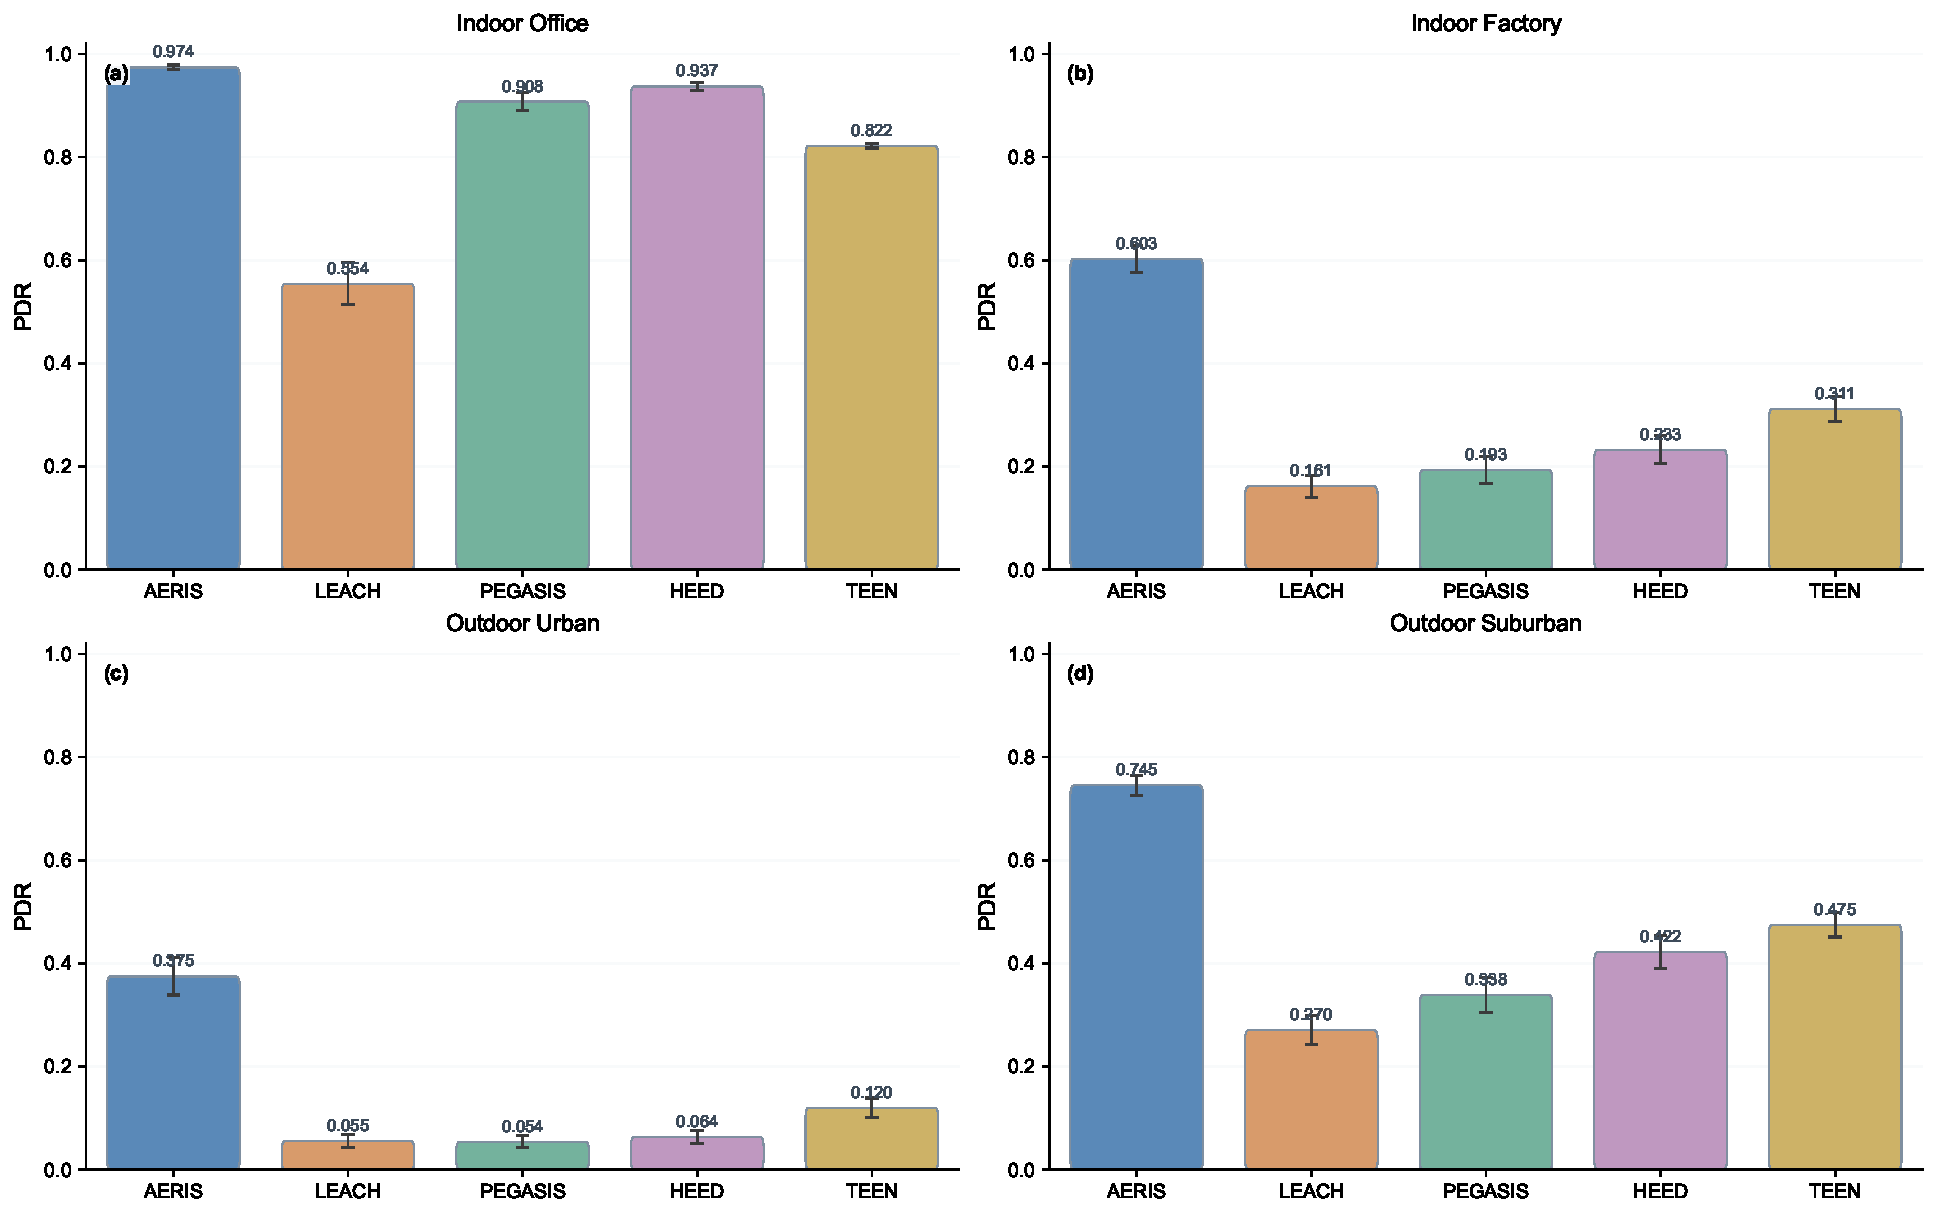
\includegraphics[width=0.95\textwidth]{fig1_env_pdr_panel_20260220_s41.pdf}
\caption{PDR comparison panel at 100 nodes (4 environments, n=30).}
\label{fig:env_panel}
\end{figure}

\subsection{Ablation: Environment-Dependent Effects (n=30)}
\begin{table}[H]
\caption{Full vs no\_gateway PDR (mean $\pm$ std; standard deviations are reported as stored in the source result file).}
\label{tab:ablation_gateway}
\centering
\begin{tabular}{lccc}
\toprule
Environment & Full & no\_gateway & Delta (no\_gateway - full) \\
\midrule
indoor\_office    & 0.9739$\pm$0.0047 & 0.9741$\pm$0.0036 & +0.0002 \\
indoor\_factory   & 0.6031$\pm$0.0258 & 0.5806$\pm$0.0215 & -0.0225 \\
outdoor\_urban    & 0.3745$\pm$0.0354 & 0.3534$\pm$0.0301 & -0.0212 \\
outdoor\_suburban & 0.7451$\pm$0.0193 & 0.7306$\pm$0.0264 & -0.0146 \\
\bottomrule
\end{tabular}
\end{table}

Gateway is positive in three environments and near-neutral in indoor\_office. CAS is not consistently positive across environments.
In indoor\_office, the Full-vs-no\_gateway gap is +0.0002 (absolute PDR), so this cell is treated as practically neutral.

\begin{figure}[H]
\centering
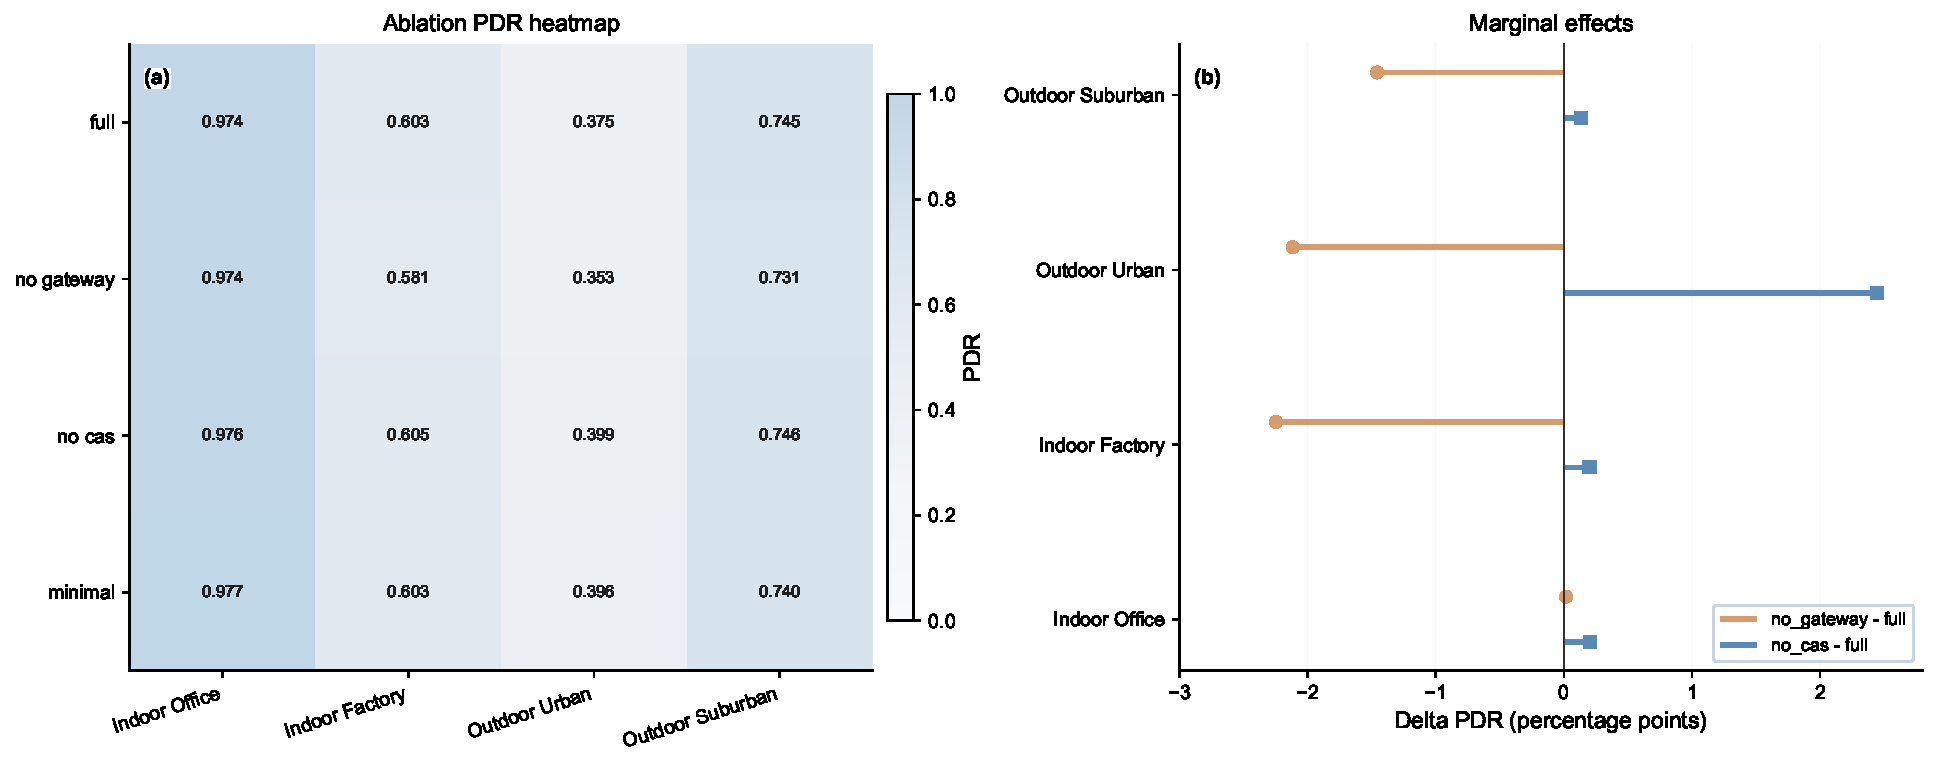
\includegraphics[width=0.95\textwidth]{fig2_ablation_panel_20260220_s41.pdf}
\caption{Ablation panel: heatmap and marginal effects (n=30).}
\label{fig:ablation_panel}
\end{figure}

\subsection{Scalability (100--1000 Nodes; Balanced n=1000 per Cell)}
\begin{table}[H]
\caption{PDR ranking at 1000 nodes from the balanced S8 frozen matrix (n=1000 per cell).}
\label{tab:scale1000}
\centering
\begin{tabular}{lcccccc}
\toprule
Environment & AERIS & LEACH & PEGASIS & HEED & TEEN & AERIS rank \\
\midrule
indoor\_office    & 0.9899 & 0.6282 & 0.8942 & 0.8915 & 0.8032 & 1st \\
indoor\_factory   & 0.9726 & 0.1884 & 0.1672 & 0.1634 & 0.2199 & 1st \\
outdoor\_urban    & 0.8846 & 0.0622 & 0.0497 & 0.0341 & 0.0662 & 1st \\
outdoor\_suburban & 0.9896 & 0.3048 & 0.2875 & 0.3232 & 0.3669 & 1st \\
\bottomrule
\end{tabular}
\end{table}

AERIS is first in all four environments in the current balanced S8 matrix under the reported simulator assumptions.
In the same S8 matrix, AERIS also shows a non-physical PDR-scale increase in three environments (indoor\_factory, outdoor\_urban, outdoor\_suburban). A plausible cause is that the original S8 simulator path omits explicit MAC-layer contention penalties, so increasing node density can artificially increase effective forwarding opportunities instead of inducing collision loss. We therefore treat S8 as a frozen baseline regime under the original simulator assumptions and use S9/S10/S11 as calibration evidence for physically stricter interpretation.
Interpretation priority in this manuscript is therefore: (i) 100-node reliability ranking, (ii) S8 as baseline scalability snapshot, and (iii) S9/S10/NS-3 as calibration and boundary evidence.

\subsection{Statistical Robustness Snapshot (AERIS vs LEACH)}
\begin{table}[H]
\caption{Holm-corrected significance snapshot at 1000 nodes (AERIS vs strongest baseline in each environment).}
\label{tab:robust_snapshot}
\centering
\begin{tabular}{lcccccc}
\toprule
Environment & Nodes & $\Delta$PDR & Hedges' $g$ & Holm $p$ & Significant \\
\midrule
indoor\_office    & 1000 & +0.095705 (vs PEGASIS) & +4.1500 & $<10^{-300}$ & yes \\
indoor\_factory   & 1000 & +0.752703 (vs TEEN) & +138.5282 & $<10^{-300}$ & yes \\
outdoor\_urban    & 1000 & +0.818370 (vs TEEN) & +180.0377 & $<10^{-300}$ & yes \\
outdoor\_suburban & 1000 & +0.622649 (vs TEEN) & +98.9577 & $<10^{-300}$ & yes \\
\bottomrule
\end{tabular}
\end{table}

This snapshot highlights strong gains in harsh environments and a moderate but significant gain in indoor\_office under the current balanced matrix.
For very large sample sizes, practical interpretation in this study still follows both effect size and absolute PDR gap rather than significance labels alone.
The very large absolute values of Hedges' $g$ in harsh environments reflect both large mean gaps and low within-group variance under large sample sizes; they should be interpreted as magnitude indicators within this experiment design, not as cross-study constants.\footnote{For large-\(n\) comparisons with very small within-group variance, standardized effect sizes can become extremely large. In this manuscript, Hedges' \(g\) is therefore interpreted jointly with absolute \(\Delta\)PDR and confidence intervals, not as a stand-alone cross-study scale.}

\begin{figure}[H]
\centering
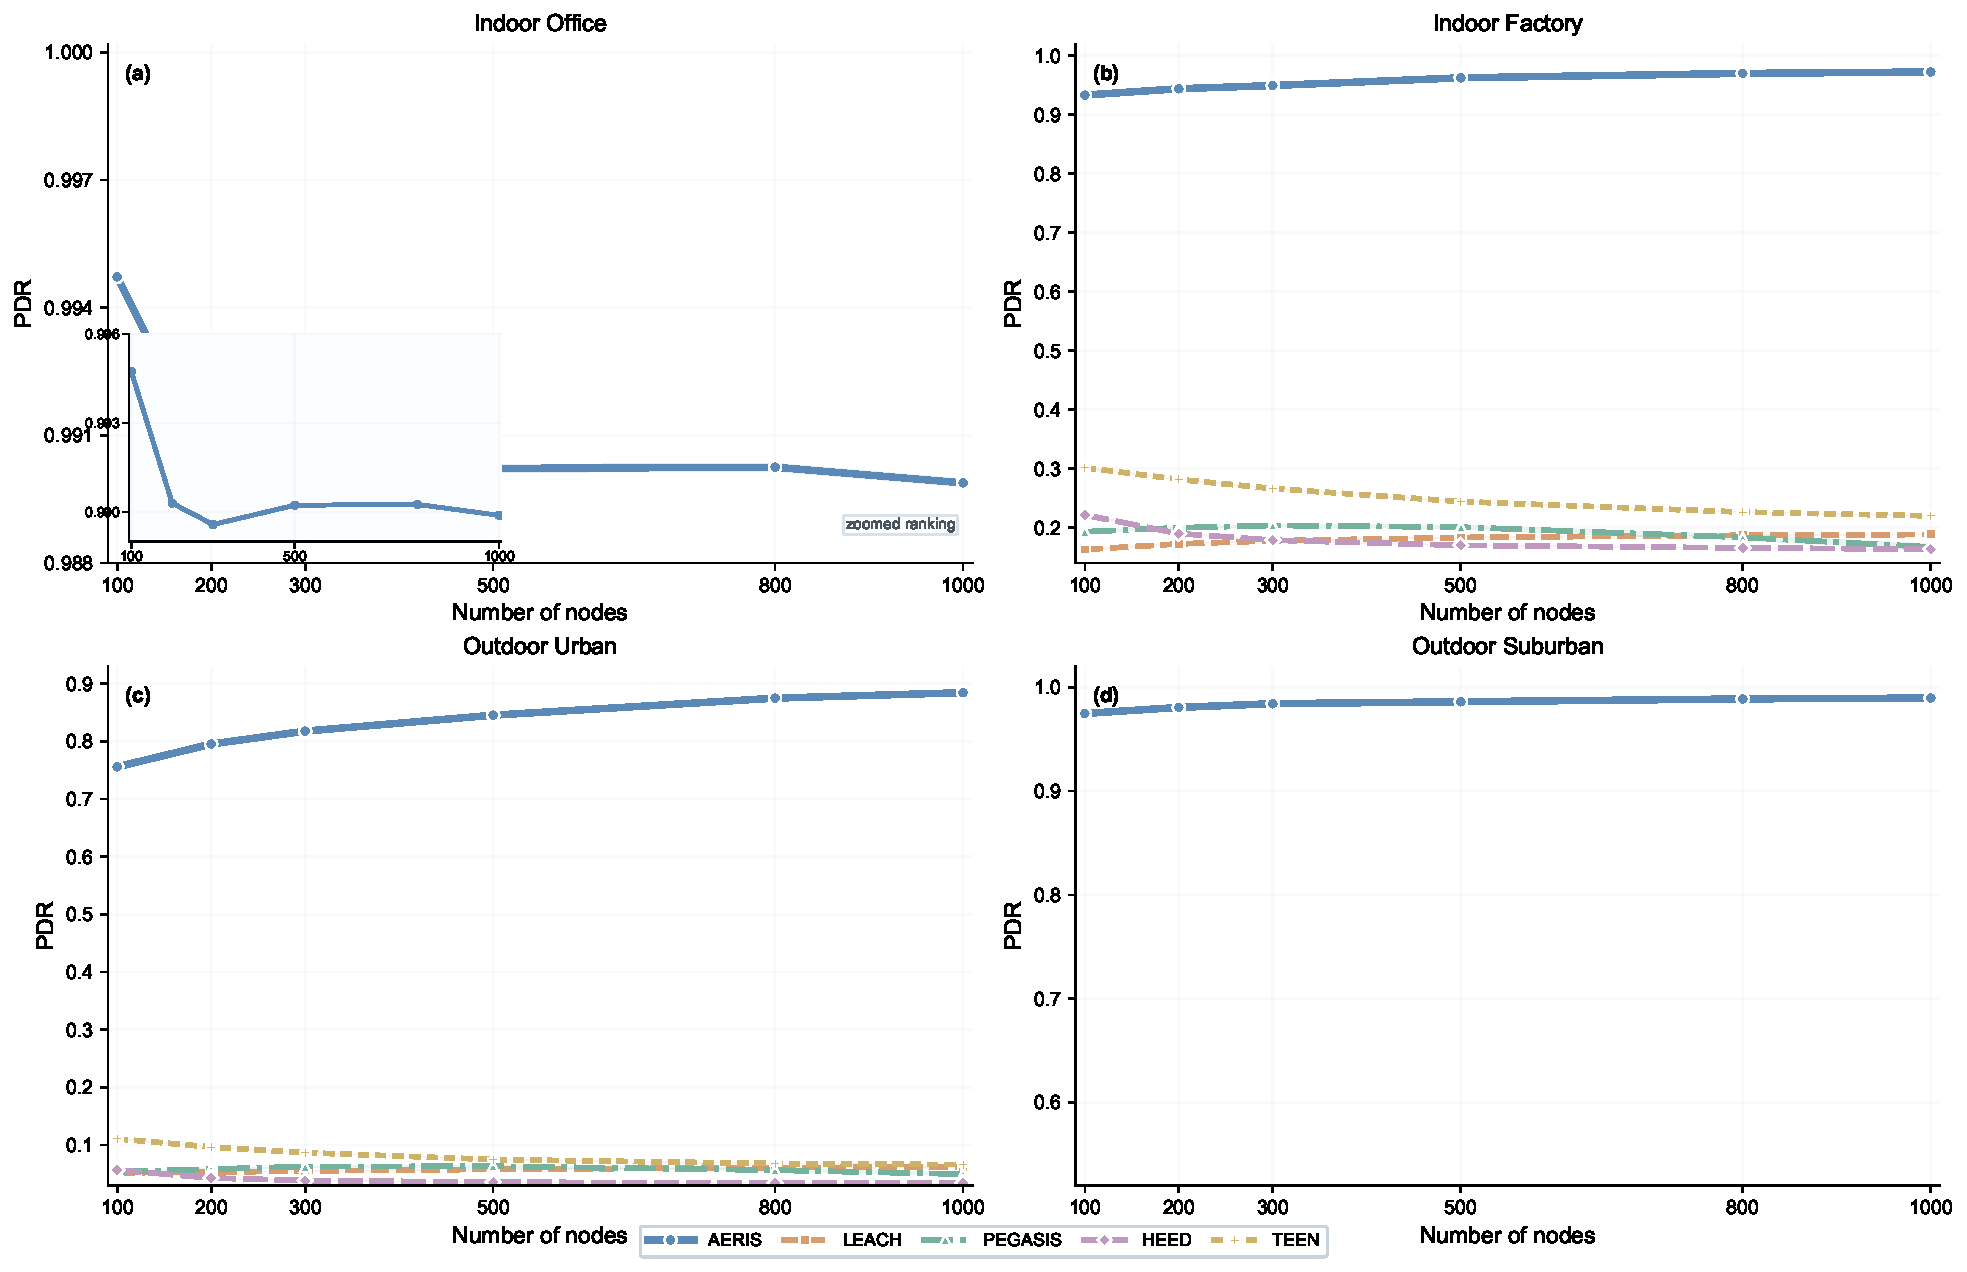
\includegraphics[width=0.95\textwidth]{fig3_scalability_panel_20260220_s41.pdf}
\caption{Scalability trends over node counts (balanced n=1000 per environment-node-protocol cell) with 95\% CI bands. The indoor\_office panel uses a narrowed y-axis window to expose non-zero ordering gaps near PDR=1.0. Under the original simulator settings (without MAC-collision modeling), AERIS exhibits an increasing trend in three environments; this is treated as a known S8 baseline limitation and is cross-checked with the stricter S9/S10 calibration blocks.}
\label{fig:scalability_panel}
\end{figure}

\subsection{Rigor-Patch Pilot Sanity Check (n=60; not used for core claims)}
To test simulator-physics consistency, we ran a publication-tier local pilot with collision and baseline multi-hop relay enabled (\texttt{--mac-collision --multihop-relay}), using the same environment taxonomy and nodes \{100, 500, 1000\} with n=60 per cell. This pilot is a sanity check and does not replace the frozen S8 matrix used for core claims.

\begin{table}[H]
\caption{AERIS PDR under the rigor-patch pilot (n=60 per environment-node cell).}
\label{tab:rigor_patch}
\centering
\begin{tabular}{lccc}
\toprule
Environment & 100 nodes & 500 nodes & 1000 nodes \\
\midrule
indoor\_office    & 0.9706 & 0.8676 & 0.6746 \\
indoor\_factory   & 0.9283 & 0.9083 & 0.7355 \\
outdoor\_urban    & 0.7487 & 0.7362 & 0.1492 \\
outdoor\_suburban & 0.9563 & 0.9193 & 0.7307 \\
\bottomrule
\end{tabular}
\end{table}

The key pilot observation is monotonicity recovery: AERIS PDR decreases with scale in all four environments. In indoor\_office, PEGASIS is higher than AERIS under this stricter setting, while AERIS remains clearly higher in the other three environments. Therefore, this pilot is treated as a gate result: it validates the direction of a simulator-rigor fix, but final paper-level scalability claims remain tied to the frozen matrix until a full rerun is completed under the upgraded simulator settings.

\subsection{Matched S9 Patch-vs-Control Stress Test (Four Environments)}
To reduce seed and sampling confounders, we ran a matched patch-versus-control stress test in all four environments (indoor\_office, indoor\_factory, outdoor\_urban, and outdoor\_suburban). The patch mode enables collision and baseline relay mechanisms; the control mode uses the original simulator path. Patch cells use n=1000 and control cells use n=600.

\begin{table}[H]
\caption{AERIS PDR in matched S9 stress test (patch vs control, four environments).}
\label{tab:s9_patch_control}
\centering
\begin{tabular}{lccc}
\toprule
Environment & Nodes & Patch & Control \\
\midrule
indoor\_office & 100  & 0.9714 & 0.9948 \\
indoor\_office & 500  & 0.8679 & 0.9902 \\
indoor\_office & 1000 & 0.6779 & 0.9899 \\
indoor\_factory & 100  & 0.9281 & 0.9329 \\
indoor\_factory & 500  & 0.9060 & 0.9627 \\
indoor\_factory & 1000 & 0.7291 & 0.9726 \\
outdoor\_urban & 100  & 0.7482 & 0.7559 \\
outdoor\_urban & 500  & 0.7299 & 0.8460 \\
outdoor\_urban & 1000 & 0.1372 & 0.8845 \\
outdoor\_suburban & 100  & 0.9556 & 0.9744 \\
outdoor\_suburban & 500  & 0.9198 & 0.9859 \\
outdoor\_suburban & 1000 & 0.7280 & 0.9897 \\
\bottomrule
\end{tabular}
\end{table}

Three observations are robust in the completed S9 evidence: (i) AERIS remains above LEACH/HEED/TEEN under patch mode in all four tested environments at 1000 nodes; (ii) PEGASIS is minimally affected by the patch, with near-zero deltas and non-significant tests in all 24 PEGASIS cells\footnote{Across the 24 PEGASIS cells in the S9 matched matrix, \(|\Delta_{\text{patch-control}}| \le 0.0044\), all Holm-adjusted \(p\)-values are \(1.0000\), and \(\max |g| = 0.0903\), consistent with a near-zero effect.}; (iii) AERIS patch-control deltas are significant in all 24 AERIS cells after Holm correction, with the largest absolute drop in outdoor\_urban at high scale. Table~\ref{tab:s9_pegasis_1000} provides a 1000-node cross-environment PEGASIS snapshot that is consistent with this stability statement. In S11, PEGASIS shows exact zero deltas in indoor\_factory (all six node counts), which is treated as an implementation-coupling anomaly pending further code-path audit rather than as physical invariance evidence. At the same time, the patch can be overly aggressive for some baseline paths at high scale, so this block is interpreted as a stress-test regime rather than a finalized replacement matrix. To remove the S9 sample-size asymmetry directly, we then run S11 as a matched confirmation block (patch \(n=1000\), control \(n=1000\) per cell) and report that matrix separately below.

\begin{table}[H]
\caption{PEGASIS patch-versus-control snapshot in S9 at 1000 nodes (n=1000 patch, n=600 control).}
\label{tab:s9_pegasis_1000}
\centering
\begin{tabular}{lcccc}
\toprule
Environment & Delta (patch-control) & Hedges' $g$ & Holm $p$ & Significant \\
\midrule
indoor\_office    & -0.0003 & -0.0435 & 1.0000 & No \\
indoor\_factory   & +0.0006 & +0.0057 & 1.0000 & No \\
outdoor\_urban    & +0.0017 & +0.0252 & 1.0000 & No \\
outdoor\_suburban & -0.0011 & -0.0085 & 1.0000 & No \\
\bottomrule
\end{tabular}
\end{table}

\subsection{S10 TX-Power Sensitivity (Four Environments)}
We additionally evaluate tx-power sensitivity under the upgraded simulation path by comparing \SI{5}{dBm} versus \SI{15}{dBm} across four environments, three node counts (100, 500, 1000), and five protocols (n=600 per cell). The full matrix contains 60 matched comparisons (4 environments $\times$ 3 node counts $\times$ 5 protocols), of which 59/60 are significant after Holm correction.

\begin{table}[H]
\caption{AERIS power-sensitivity snapshot at 1000 nodes (S10, metric=\texttt{pdr\_expected}).}
\label{tab:s10_aeris_1000}
\centering
\begin{tabular}{lccc}
\toprule
Environment & tx=\SI{5}{dBm} & tx=\SI{15}{dBm} & Delta (5--15) \\
\midrule
indoor\_office    & 0.8177 & 0.5367 & +0.2810 \\
indoor\_factory   & 0.6623 & 0.5051 & +0.1571 \\
outdoor\_urban    & 0.0587 & 0.1606 & -0.1019 \\
outdoor\_suburban & 0.7679 & 0.5440 & +0.2239 \\
\bottomrule
\end{tabular}
\end{table}

\begin{figure}[H]
\centering
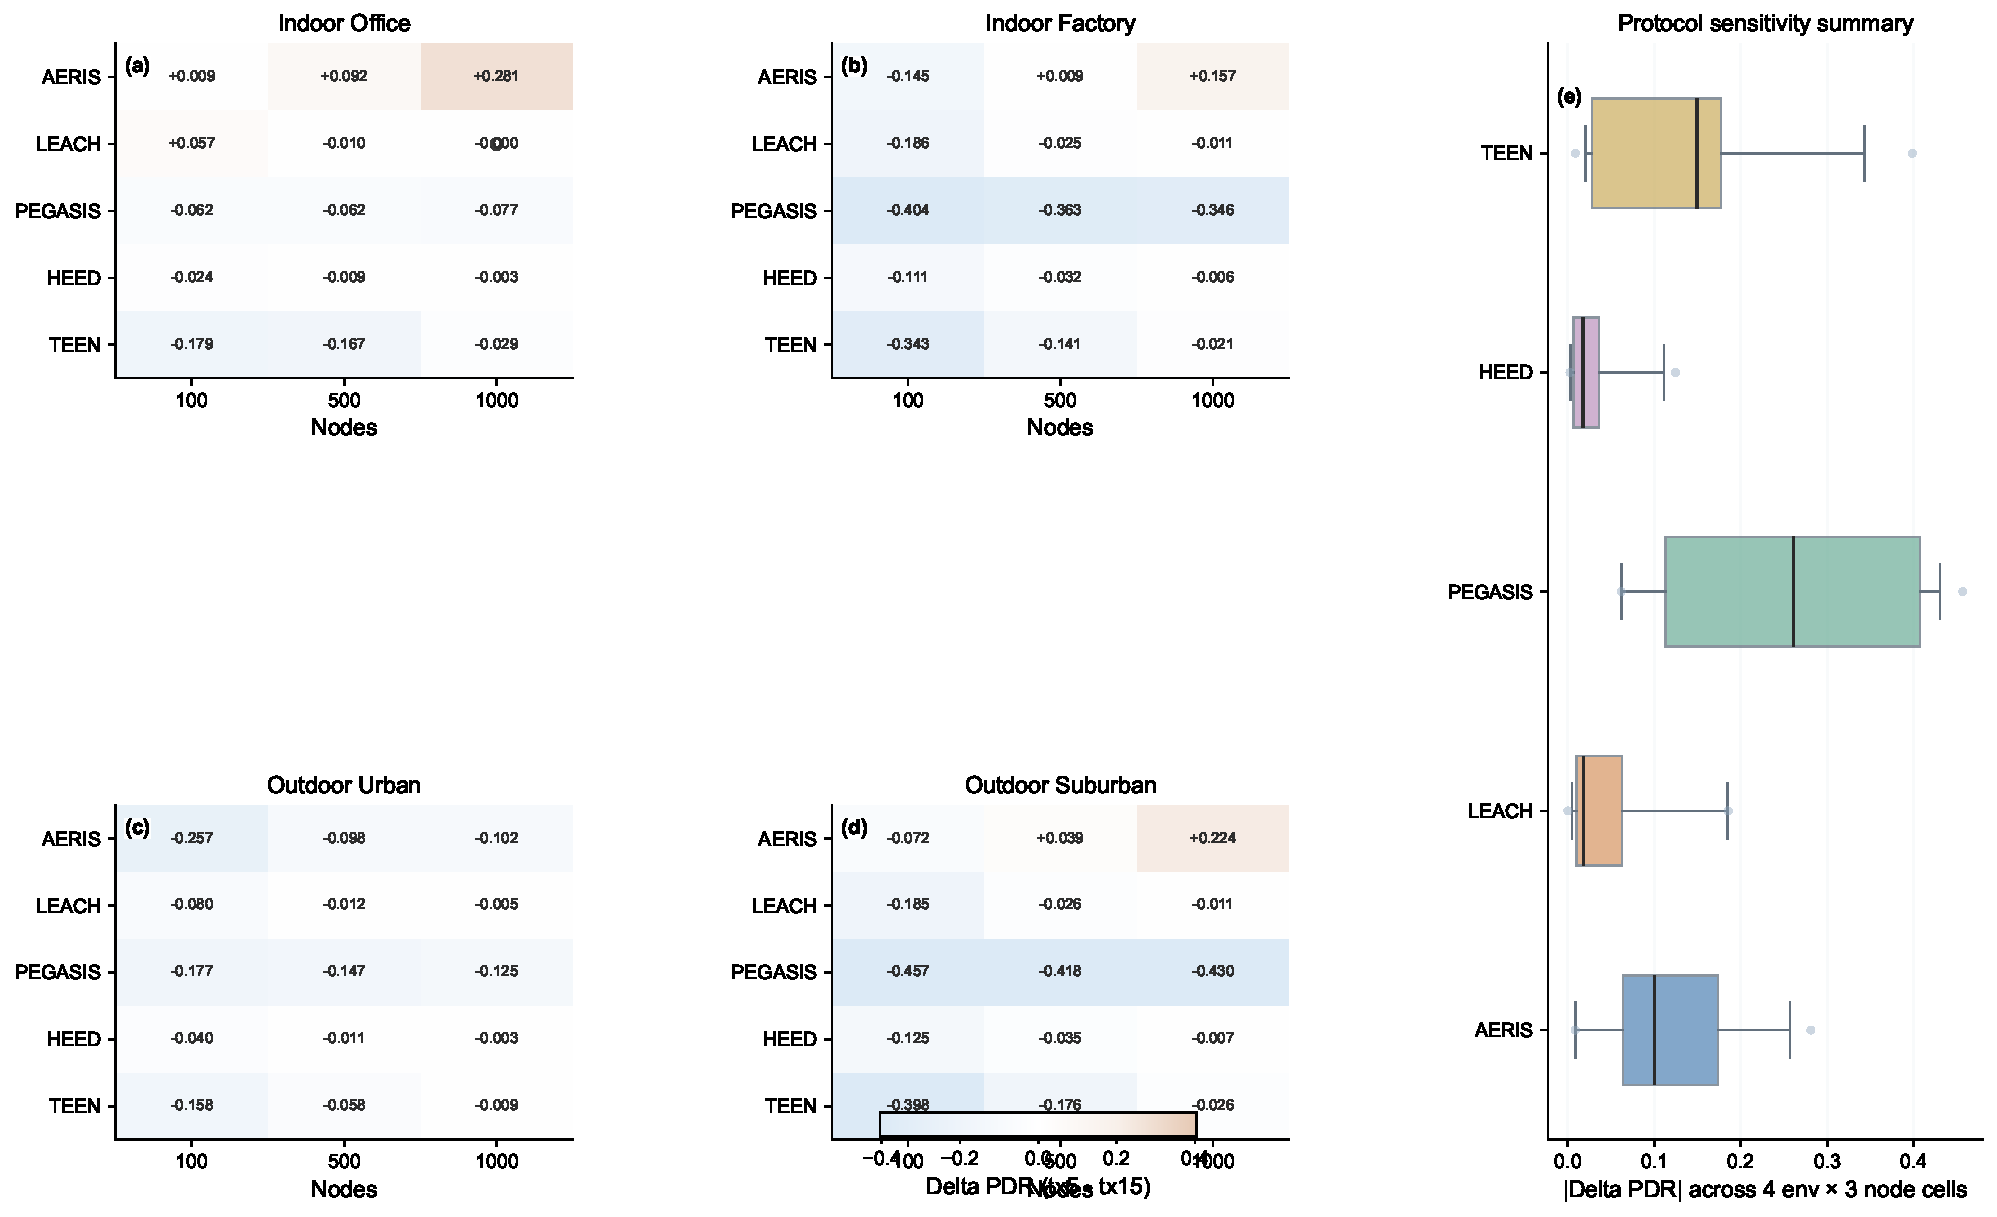
\includegraphics[width=0.95\textwidth]{fig6_s10_power_sensitivity_20260220_s41.pdf}
\caption{S10 full-matrix power sensitivity (tx5 vs tx15). Panels (a)--(d) show per-environment protocol-by-scale delta maps (\(\Delta\)PDR = tx5 -- tx15) for all 60 tested cells; hollow markers denote non-significant cells after Holm correction. Panel (e) summarizes protocol-level absolute sensitivity across 4 environments \(\times\) 3 node scales.}
\label{fig:s10_power_sensitivity}
\end{figure}

The S10 block confirms that power response is environment-dependent and non-monotonic under the current routing and channel settings. In particular, raising tx-power does not guarantee higher PDR in every environment-node cell. The single non-significant comparison in the 60-cell matrix is LEACH at indoor\_office, 1000 nodes, while all other 59 cells are significant after Holm correction.

\subsection{S11 Matched Patch-vs-Control Matrix (Four Environments, n=1000 vs 1000)}
To remove remaining sample-size asymmetry from S9, we completed a fully matched S11 matrix in which both patch and control arms use n=1000 per environment-node-protocol cell (4 environments $\times$ 6 node counts $\times$ 5 protocols). This block directly tests whether stricter physics assumptions improve or degrade reliability under matched sampling.

\begin{table}[H]
\caption{AERIS patch-control deltas in the completed S11 matched matrix (delta = patch - control).}
\label{tab:s11_aeris_delta}
\centering
\begin{tabular}{lcc}
\toprule
Environment & Delta at 100 nodes & Delta at 1000 nodes \\
\midrule
indoor\_office    & -0.0234 & -0.3120 \\
indoor\_factory   & -0.0052 & -0.2435 \\
outdoor\_urban    & -0.0077 & -0.7474 \\
outdoor\_suburban & -0.0191 & -0.2616 \\
\bottomrule
\end{tabular}
\end{table}

In the S11 matched matrix, AERIS patch-control deltas are negative and significant in all 24 environment-scale cells after Holm correction (24/24 significant; Hedges' $g$ range: -0.47 to -15.36). Therefore, under the current patch configuration (\texttt{mac-collision + multihop-relay}), stricter physics assumptions reduce reliability rather than increase it. This means the patch block is evidence for realism stress, not yet evidence for superior calibrated performance.

\begin{figure}[H]
\centering
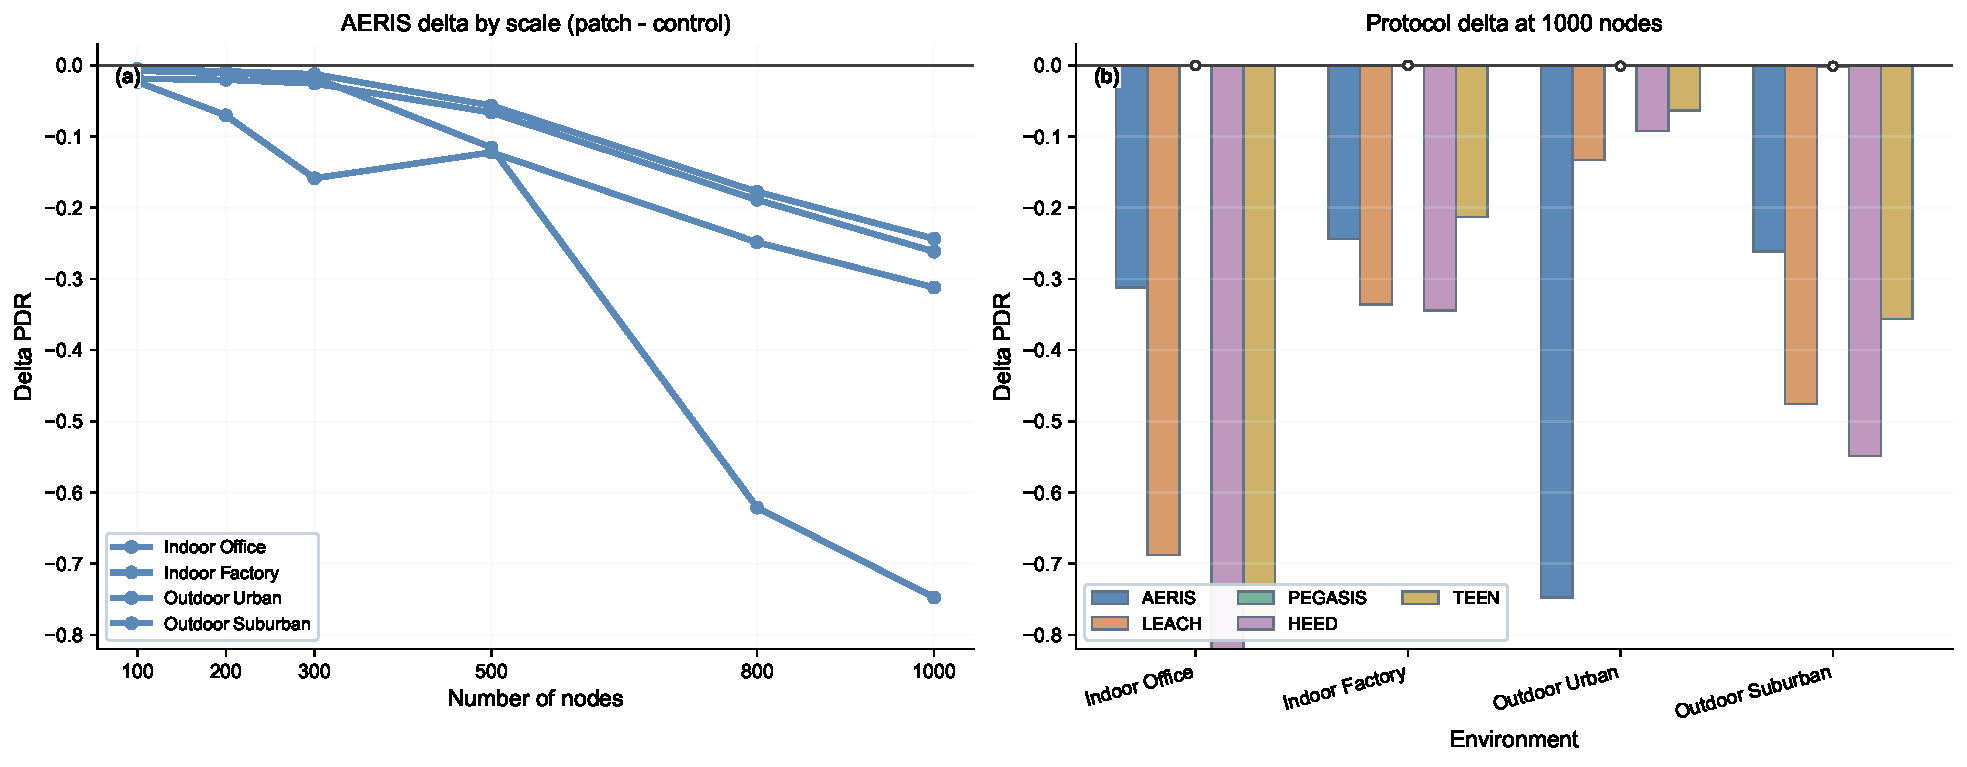
\includegraphics[width=0.95\textwidth]{fig5_s11_patch_control_delta_20260220_s41.pdf}
\caption{S11 matched patch-control evidence. (a) AERIS delta trajectories over node counts (patch - control). (b) Protocol deltas at 1000 nodes across environments. Negative deltas indicate lower PDR under patch mode.}
\label{fig:s11_patch_control}
\end{figure}

\subsection{Hop-Based Latency and Trade-offs}
At 100 nodes (n=30), AERIS stays near two hops (1.97--1.99), while PEGASIS remains above 31 hops due to chain traversal. LEACH and TEEN show lower average hops because of protocol paths that allow direct-to-BS transmissions.

\begin{figure}[H]
\centering
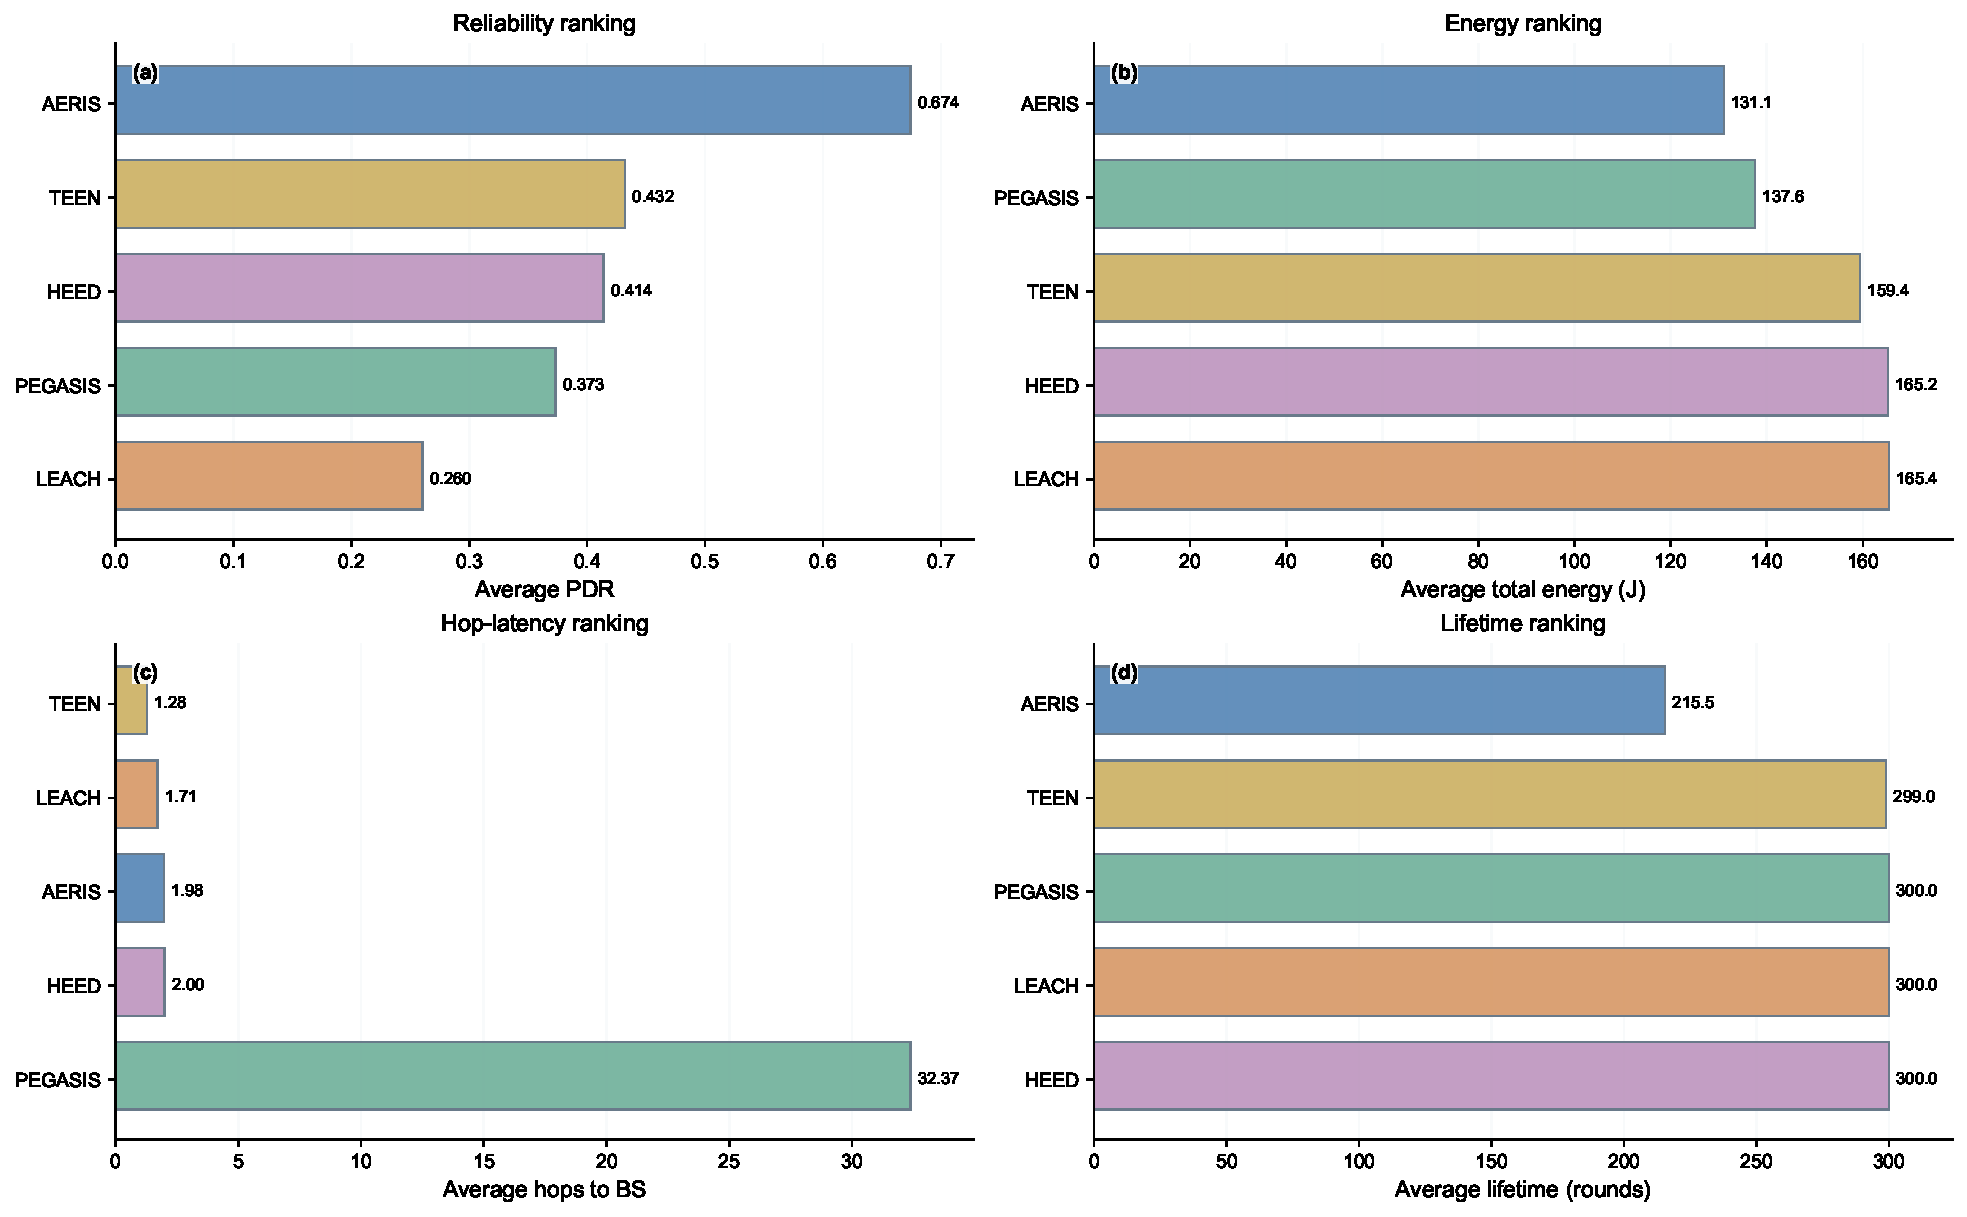
\includegraphics[width=0.95\textwidth]{fig4_tradeoff_panel_20260220_s41.pdf}
\caption{Trade-off panel from publication-tier data: reliability, energy, hop-based latency, and lifetime. The hop panel uses a logarithmic x-axis to keep low-hop and high-hop protocols visible in the same frame without overlap.}
\label{fig:tradeoff_panel}
\end{figure}

\subsection{NS-3 Trend Validation (AERIS vs LEACH, n=30)}
NS-3 validation is used as a cross-platform trend check rather than a numerical-equivalence proof. This block is restricted to AERIS-versus-LEACH and is not used for five-protocol cross-platform ranking. Under aligned multi-environment settings, AERIS is directionally not lower than LEACH in 27 of 28 tested environment-scale cells; the single exception is indoor\_office at 200 nodes (AERIS--LEACH diff $=-0.0004$, not significant). At 100 nodes, significance is confirmed in 3/4 environments (indoor\_factory, outdoor\_urban, outdoor\_suburban), while indoor\_office remains non-significant. In the 300/500-node extension, all eight environment-scale comparisons are significant after Holm correction; with the 800/1000 extension included, non-significance remains confined to indoor\_office at 1000 nodes.

\begin{table}[H]
\caption{NS-3 trend-level validation at 100 nodes (AERIS vs LEACH, n=30; metric=\texttt{pdr\_expected}).}
\label{tab:ns3_trend}
\centering
\begin{tabular}{lccccc}
\toprule
Environment & AERIS & LEACH & Delta & Holm-corrected $p$ & Significance \\
\midrule
indoor\_office    & 0.9202 & 0.9185 & +0.0017 & 1.00 & no \\
indoor\_factory   & 0.6025 & 0.5336 & +0.0690 & $4.23\times10^{-25}$ & yes \\
outdoor\_urban    & 0.2064 & 0.1899 & +0.0165 & $3.41\times10^{-3}$ & yes \\
outdoor\_suburban & 0.7771 & 0.6921 & +0.0850 & $1.94\times10^{-30}$ & yes \\
\bottomrule
\end{tabular}
\end{table}

\begin{figure}[H]
\centering
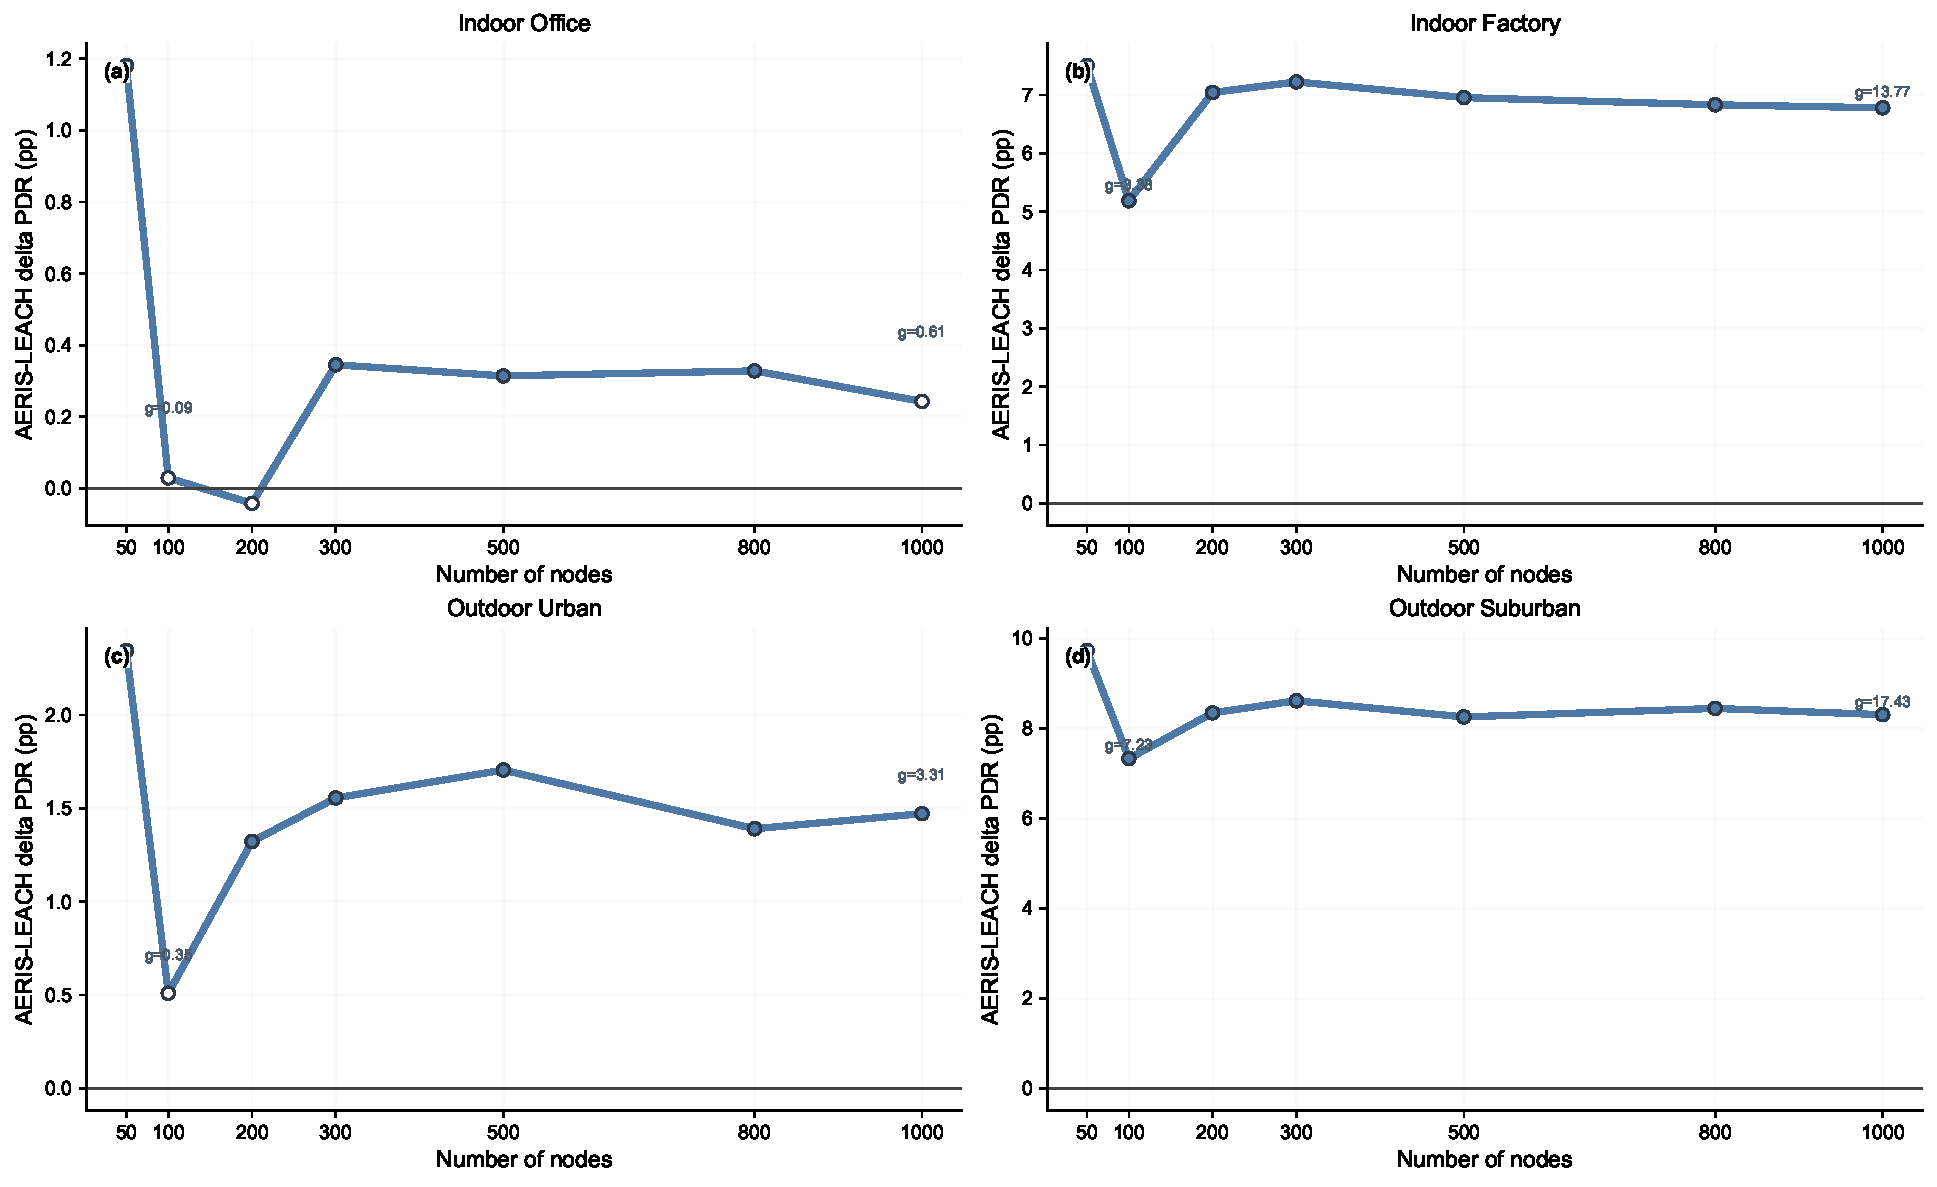
\includegraphics[width=0.95\textwidth]{fig7_ns3_trend_panel_20260220_s41.pdf}
\caption{NS-3 trend panel over 50--1000 nodes (AERIS--LEACH delta in percentage points). Hollow markers denote non-significant cells after Holm correction.}
\label{fig:ns3_trend_panel}
\end{figure}

Scope note: this NS-3 block supports trend consistency only. The manuscript does not claim cross-platform numerical equivalence. Across 7 node counts and 4 environments, 25/28 AERIS-versus-LEACH comparisons are significant; the non-significant cells are indoor\_office at node counts 100, 200, and 1000.

\section{Discussion}
The evidence supports environment-scoped positioning rather than universal superiority. In the reported matrices, AERIS is strongest on reliability in harsh channels.

The manuscript separates three evidence blocks:
\begin{itemize}
\item 100-node multi-environment comparison,
\item large-scale regime (100--1000 nodes) with balanced n=1000 per cell,
\item NS-3 trend validation for AERIS versus LEACH only.
\end{itemize}
Cross-block numerical pooling is avoided because these blocks answer different questions. Under stricter S9/S11 collision-relay settings, high-scale PDR decreases for most protocols and PEGASIS remains comparatively stable. Under S10, tx-power effects are strong but not globally monotonic. Practical interpretation therefore remains environment-scoped.

Practical interpretation also requires separating statistical and engineering significance. At large sample sizes, very small absolute differences can be significant after correction. For this reason, we interpret each result jointly by corrected $p$ value, effect size, and absolute PDR delta. Energy interpretation is similarly conditioned: lower total energy can co-occur with shorter lifetime when earlier network termination occurs.

\subsection*{Practical Deployment Guidance}
Based on the completed matrices, the following deployment guidance is supported by the reported evidence:
\begin{itemize}
\item In harsh environments (indoor\_factory, outdoor\_urban, outdoor\_suburban), enabling Gateway support is recommended because no-gateway ablations reduce reliability.
\item In benign indoor\_office conditions, gains are smaller and model overhead should be justified against application reliability targets.
\item For high-scale deployments, treat S8 as baseline evidence and use S9/S10/S11 calibration before final engineering parameter selection.
\item Tx-power settings should be environment-tuned; monotonic power assumptions are not supported by S10.
\end{itemize}

\begin{table}[H]
\caption{Environment-scoped engineering interpretation from the reported evidence.}
\label{tab:deployment_summary}
\centering
\small
\begin{tabular}{>{\raggedright\arraybackslash}p{0.24\textwidth} >{\raggedright\arraybackslash}p{0.42\textwidth} >{\raggedright\arraybackslash}p{0.26\textwidth}}
\toprule
Environment type & Recommended interpretation & Main caveat \\
\midrule
indoor\_office & Reliability gaps are small at high scale; deployment cost and simplicity can dominate design choice & Some NS-3 cells are non-significant \\
indoor\_factory & AERIS with Gateway support gives the most stable reliability gain & Calibrate tx-power and collision parameters \\
outdoor\_urban & AERIS remains preferable under harsh links in both simulator regimes & High-scale behavior is sensitive to physics settings \\
outdoor\_suburban & AERIS trend remains favorable in simulator and NS-3 trend checks & Do not assume monotonic power-response \\
\bottomrule
\end{tabular}
\normalsize
\end{table}

\subsection*{Reviewer-Critical Validity Notes}
Three validity boundaries are explicit in this draft. First, the reported comparisons are simulator-based under the tested channel taxonomy. Second, NS-3 evidence is trend-level only. Third, module contributions are context dependent: Gateway and CAS effects vary by environment and should not be interpreted as globally monotonic benefits.

\section{Limitations and Future Work}
\begin{itemize}
\item Current evidence is simulator-based.
\item NS-3 trend-level publication gate is completed; numerical equivalence is outside the current validation scope.
\item NS-3 validation in this manuscript focuses on AERIS versus LEACH; full five-protocol cross-platform ranking remains future work.
\item The large-scale S8 matrix is balanced at n=1000 per cell and should be interpreted under the original simulator assumptions.
\item A matched S9 patch-versus-control stress test has now been completed in all four environments (patch n=1000, control n=600 per environment-node-protocol cell); unequal sample sizes come from phased execution and are handled with Welch's test.
\item A fully matched S11 patch-versus-control matrix has also been completed (patch n=1000, control n=1000 per environment-node-protocol cell); AERIS deltas are negative and significant in all 24 environment-scale cells under the current patch configuration.
\item A matched S10 tx-power sensitivity matrix has now been completed in all four environments (tx=\SI{5}{dBm} vs \SI{15}{dBm}, n=600 per environment-node-protocol cell); 59/60 cells are significant, but response direction is environment-dependent.
\item Under patch mode, high-scale baseline PDR can become very low in benign channels, so collision/relay parameter calibration is still required before replacing the frozen S8 matrix in the final camera-ready version.
\item Reported gains are limited to the tested baseline set and channel taxonomy.
\item Hop count is reported as a route-length proxy, not as a wall-clock latency benchmark under full MAC scheduling.
\item Additional topology families (corridor, hotspot) and hardware-in-the-loop validation remain pending.
\end{itemize}

\section{Conclusion}
AERIS provides a reliability-oriented routing option for heterogeneous WSN channels. In the publication-tier 100-node matrix, it achieves the highest mean PDR within the tested baseline set across all four environments. In the balanced S8 large-scale matrix (100--1000 nodes, n=1000 per cell), AERIS is the highest-mean protocol in all tested environments; however, S8 is treated as baseline evidence because it excludes MAC-collision modeling and shows non-physical upward trends in three environments.

NS-3 adds trend-level support for AERIS versus LEACH. The completed S9 stress block, S10 power-sensitivity matrix, and S11 fully matched patch-control matrix show that stricter physics and power changes can materially alter high-scale behavior; in S11, AERIS patch-control deltas are negative and significant in all 24 environment-scale cells under the current patch setup. Collision/relay parameter calibration is therefore required before replacing S8 with a finalized publication scalability matrix.

The practical takeaway is therefore conditional: AERIS is strong for reliability-first deployments in harsh channels, while final high-scale parameterization must be selected under calibrated collision/relay settings rather than transferred directly from frozen baseline matrices.

\authorcontributions{Conceptualization, X.Z. and K.L.; methodology, K.L. and J.L.; software, K.L.; validation, X.Z. and J.L.; writing---original draft preparation, K.L.; writing---review and editing, X.Z.; supervision, X.Z.}
\funding{This research received no external funding.}
\conflictsofinterest{The authors declare no conflict of interest.}
\section*{Data Availability Statement}
The datasets, scripts, manuscript sources, figure-generation code, and provenance sidecar records (including commit identifiers and script hashes) supporting this study are available from the corresponding author and will be released in a versioned public repository upon final publication. The released archive includes the full 100-node benchmark matrix, the frozen S8 scalability matrix and significance tables, S9/S10/S11 calibration matrices, and the NS-3 trend-level validation summary.

\reftitle{References}
\bibliography{bibliography}

\end{document}
